{\bf Test Cases}

The autograder is a thin wrapper over the python |unittest| framework.  It can
be run either locally (on your computer) or remotely (on SCPD servers).  The
following description demonstrates what test results will look like for both
local and remote execution.  For the sake of example, we will consider two
generic tests: |1a-0-basic| and |1a-1-hidden|.

{\bf Local Execution - Hidden Tests}

All hidden tests rely on files that are not provided to students.  Therefore,
the tests can only be run remotely.  When a hidden test like |1a-1-hidden| is
executed locally, it will produce the following result:

\begin{center}
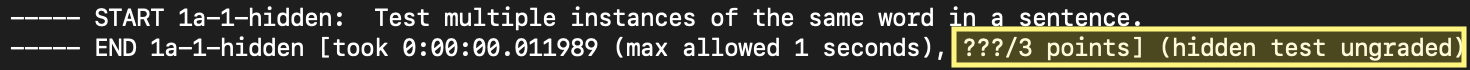
\includegraphics[width=1\textwidth]{00-instructions/local-hidden.png}
\end{center}

{\bf Local Execution - Basic Tests}

When a basic test like |1a-0-basic| passes locally, the autograder will indicate
success:

\begin{center}
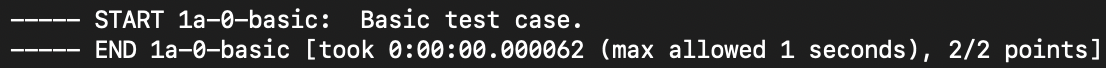
\includegraphics[width=1\textwidth]{00-instructions/local-basic-passed.png}
\end{center}

When a basic test like |1a-0-basic| fails locally, the error is printed to the
terminal, along with a stack trace indicating where the error occurred:

\begin{center}
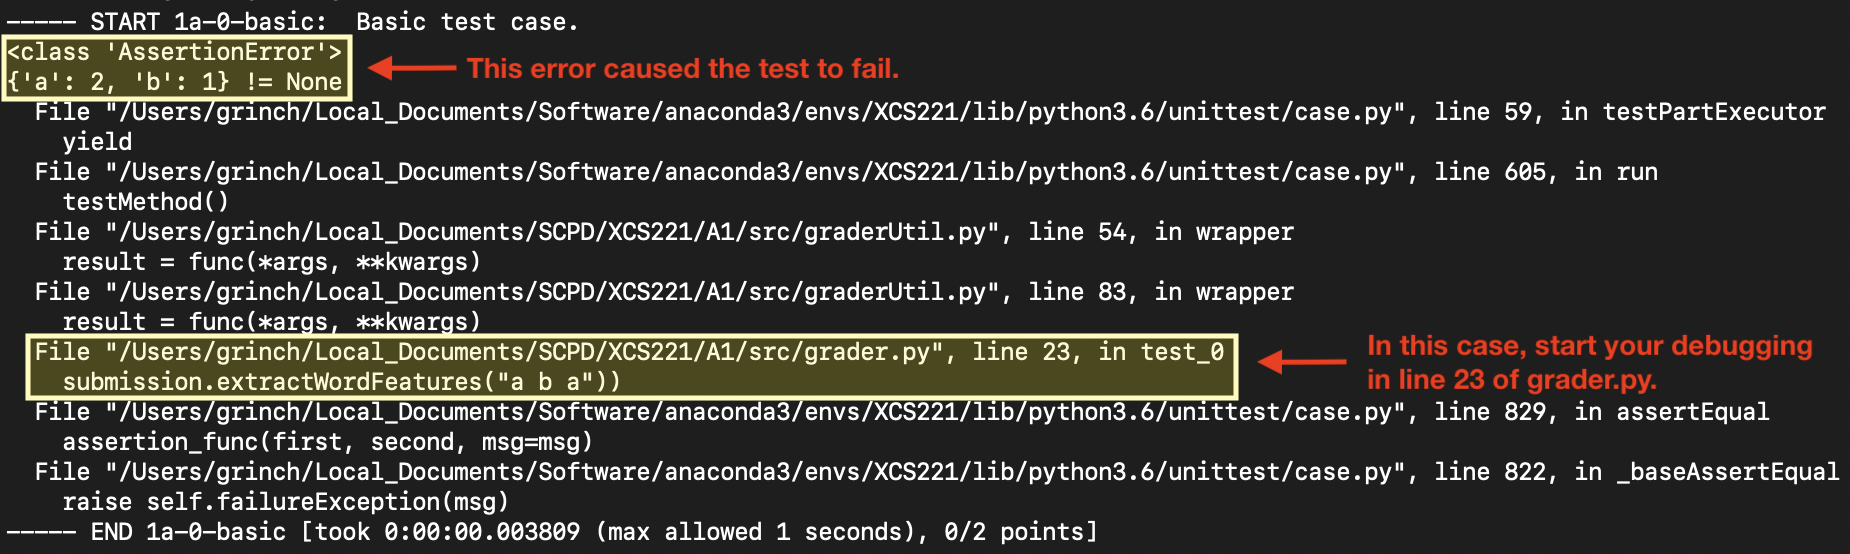
\includegraphics[width=1\textwidth]{00-instructions/local-basic-failed.png}
\end{center}

{\bf Remote Execution}

Basic and hidden tests are treated the same by the remote autograder.  Here are
screenshots of failed basic and hidden tests.  Notice that the same information
(error and stack trace) is provided as the in local autograder, now for both
basic and hidden tests.

\begin{center}
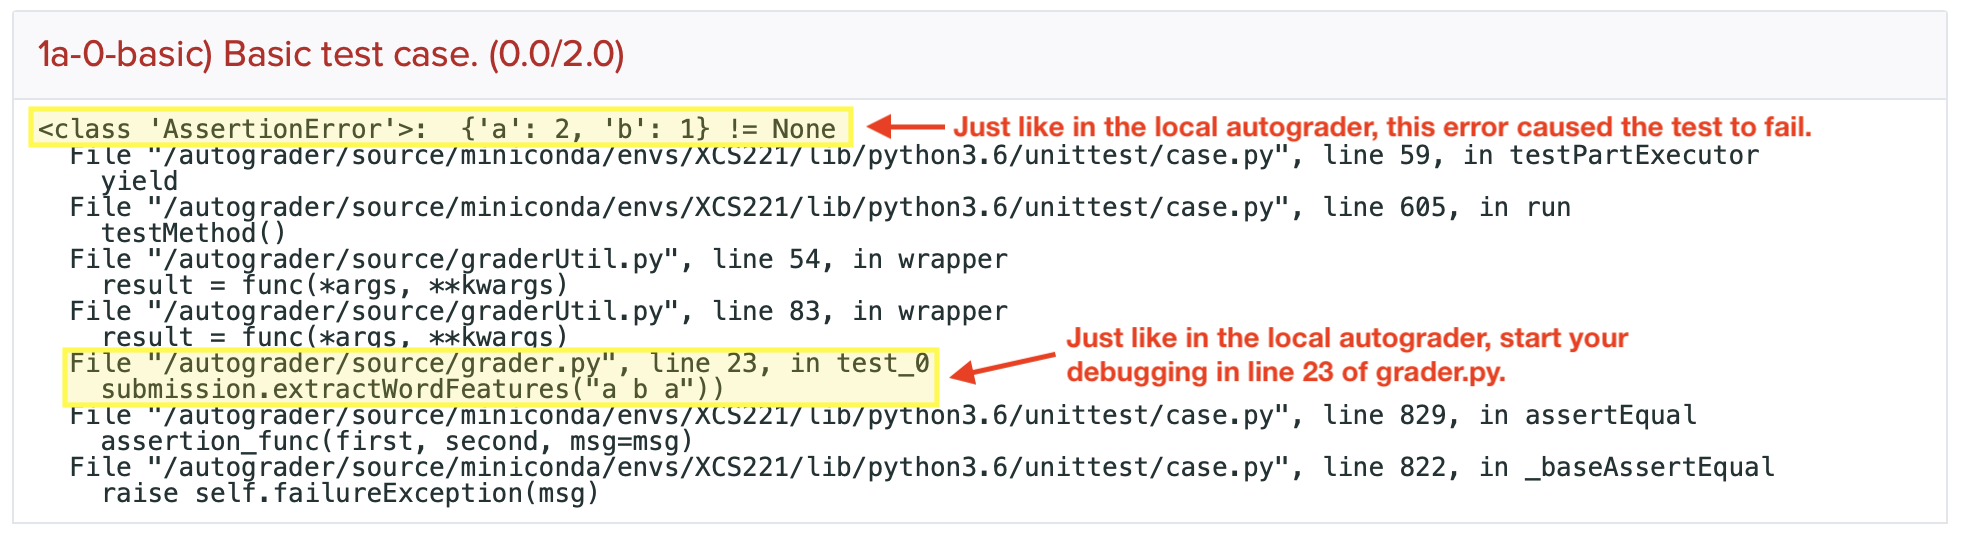
\includegraphics[width=1\textwidth]{00-instructions/remote-basic-failed.png}
\end{center}

\begin{center}
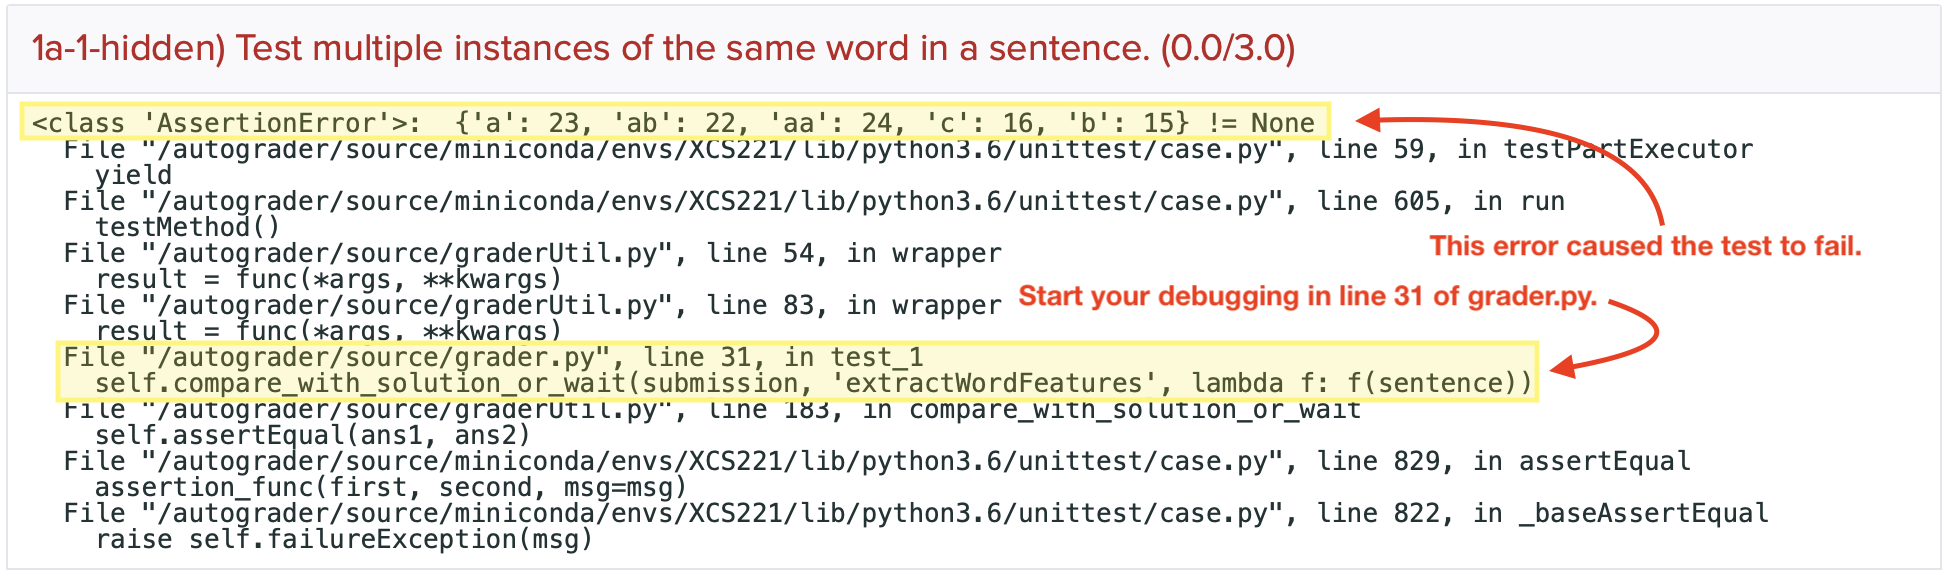
\includegraphics[width=1\textwidth]{00-instructions/remote-hidden-failed.png}
\end{center}

Finally, here is what it looks like when basic and hidden tests pass in the
remote autograder.

\begin{center}
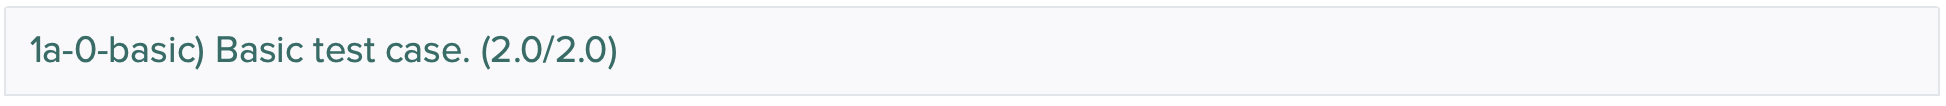
\includegraphics[width=1\textwidth]{00-instructions/remote-basic-passed.png}
\end{center}

\begin{center}
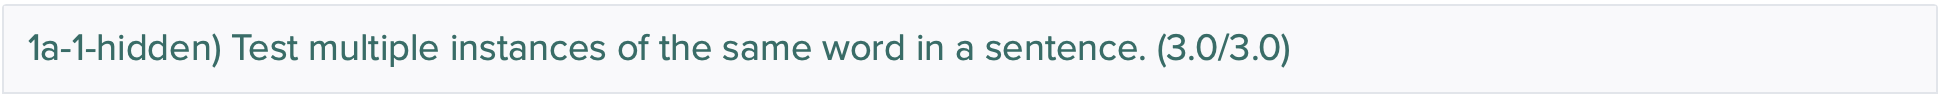
\includegraphics[width=1\textwidth]{00-instructions/remote-hidden-passed.png}
\end{center}
